\documentclass{article}

\usepackage{ragged2e}
\usepackage{graphicx}
\usepackage{caption}
\usepackage{tikz}
\usepackage{titling}
\usepackage{enumitem}
\usepackage{palatino}
\usepackage{setspace}
\usepackage[top=3.5cm, right=3.5cm, bottom=3.5cm, left=3.5cm]{geometry}
\usetikzlibrary{automata, positioning, arrows}

\captionsetup{font=footnotesize}
\setlength\parindent{0pt}
\linespread{1.05}

\begin{document}

\begin{titlepage}
    \vspace*{-\topskip}
    %\hrule
    \centering

    %
    \vspace{0.5cm} {
        \normalsize Politecnico di Milano \\ Dipartimento di Elettronica, Informazione e Bioingegneria
    }

    % date
    \vspace{5cm}
    {
        \large
        15 Luglio 2024
        \par
    }
    
    % title
    \vspace{0.25cm}
    {
        \LARGE
        \textbf{Prova Finale di Reti Logiche \\ 2023 - 2024}
        \par
    }
    
    % table with content
    \vspace{1.5cm}
    {
        \noindent
        \begin{center}
            \large
            \begin{tabular}{l r}
                Studente: & Andrea Sanvito \\
                Matricola: & 983819 \\
                Codice Persona: & 10814394 \\
                \\
                Docente: & Gianluca Palermo \\
            \end{tabular}
        \end{center}
    }

    % polimi badge
    \vspace{4.25cm}
    {
        \includegraphics[width=0.6\textwidth]{polimi_badge.png}
    }
    
    \vfill
    \vspace*{-3.5cm}
    %\hrule
\end{titlepage}


%---------------------------
%         Section 1
%---------------------------

\section{Requisiti del Progetto}
\subsection{Descrizione del problema}
Il progetto riguarda l'implementazione in VHDL di un modulo in grado di modificare valori all'interno di una memoria RAM, seguendo determinate specifiche.
\bigskip
\\ Viene dato in input al modulo un indirizzo da 16 bit della memoria \texttt{i\_add} e un valore intero \texttt{i\_k} da 10 bit.
Il compito del modulo è di:
\begin{itemize}[label=\raisebox{0.25ex}{\tiny$\bullet$}]
    \item accedere alla memoria all'indirizzo \texttt{i\_add} fornito in input;
    \item intendere la memoria come una sequenza di "coppie" di numeri, dove il primo rappresenta un dato, e il secondo un
    valore di credibilità del dato stesso.
    \item scorrere le \texttt{i\_k} coppie in memoria una ad una, e ad ogni passo:
    \begin{enumerate}[label=\roman*.]
        \item se il dato è specificato (ossia diverso da zero), lo si mantiene in memoria e si imposta il valore di credibilità seguente al massimo;
        \item altrimenti, si aggiorna il dato in memoria con l'ultimo dato valido letto, e si decrementa il valore di credibilità.
    \end{enumerate}
\end{itemize}

L'implementazione deve essere completamente sincrona con un segnale di clock fornito esternamente, eccetto per il segnale di reset, il quale è invece asincrono.

\vspace{0.5cm}
\subsection{Ipotesi Progettuali}
Il progetto è stato svolto con determinate ipotesi:
\begin{enumerate}[label=\roman*.]
    \item l'indirizzo \texttt{i\_add} deve essere valido, ossia non deve superare la dimensione della me-moria;
    \item la somma tra \texttt{i\_add} e \texttt{i\_k} deve essere valida, ossia non deve superare la dimensione della memoria;
\end{enumerate}
Il comportamento del modulo implementato non è specificato per i casi sopra elencati.
\bigskip \\ Inoltre, per quanto riguarda i segnali di start asseriti durante un segnale di reset, si è interpretato dalle specifiche che il modulo debba attendere un nuovo segnale di start. Di conseguenza, il modulo non avvierà l'elaborazione con lo stesso segnale di start asserito durante il reset.
\bigskip \\ E' riportato di seguito un esempio di elaborazione.

\vspace{0.5cm}
\subsection{Esempio}
Consideriamo l'indirizzo di memoria iniziale \texttt{i\_add} pari a 127 e \texttt{i\_k} pari a 16.

\begin{figure}[h]
    \centering
    \includegraphics[width=0.65\textwidth]{example.png}
    \caption[short]{memoria RAM prima e dopo le operazioni svolte dal modulo}
\end{figure}

\bigskip
Il nostro modulo accede in lettura alla memoria all'indirizzo specificato: essendo il dato diverso da zero, lo salva come ultimo valore valido e porta il valore di credibilità al massimo (da specifica, il massimo equivale a 31), scrivendolo nella cella seguente.

\newpage
La cella successiva a quella appena scritta contiene uno zero, ossia un valore non specificato: il modulo lo sostituisce inserendo l'ultimo valore valido, e decrementa la credibilità, scrivendola nella cella successiva. 
\bigskip \\ Questo processo continua fino alla cella all'indirizzo 133, dove viene trovato un dato diverso da zero. Il modulo procede ad aggiornare il proprio ultimo valore valido letto, e a riportare la credibilità a 31, scrivendola nella cella successiva.
\bigskip \\ Tali azioni si ripetono fino a quando il contatore \texttt{k}, decrementato ad ogni lettura, raggiunge lo zero.


%---------------------------
%         Section 2
%---------------------------

\newpage
\section{Architettura}
\subsection{Specifica}
La specifica del problema richiede che la soluzione includa un componente con la seguente interfaccia:

\begin{figure}[h]
    \centering
    \includegraphics[width=0.6\textwidth]{interface.png}
\end{figure}

Il modulo deve dunque comunicare con altre entità, in particolare:
\begin{itemize}[label=\raisebox{0.25ex}{\tiny$\bullet$}]
    \item un utilizzatore, attraverso i segnali in input \texttt{i\_clk}, \texttt{i\_rst}, \texttt{i\_start}, \texttt{i\_add}, \texttt{i\_k};
    \item una memoria RAM, sfruttando i segnali in output \texttt{o\_mem\_addr}, \texttt{o\_mem\_data}, \texttt{o\_mem\_we}, \texttt{o\_mem\_en}, e un segnale in input \texttt{i\_mem\_data}.
\end{itemize}
E' anche utilizzato un segnale in output \texttt{o\_done} per comunicare all'utilizzatore la fine dell'ela\-borazione da parte del modulo.

\subsection{Finite State Machine}
L'implementazione è stata ottenuta attraverso un singolo modulo, una FSM, con due processi.
Essa comunica con la memoria, esegue computazione, e asserisce gli output.

\begin{figure}[ht]
    \centering
    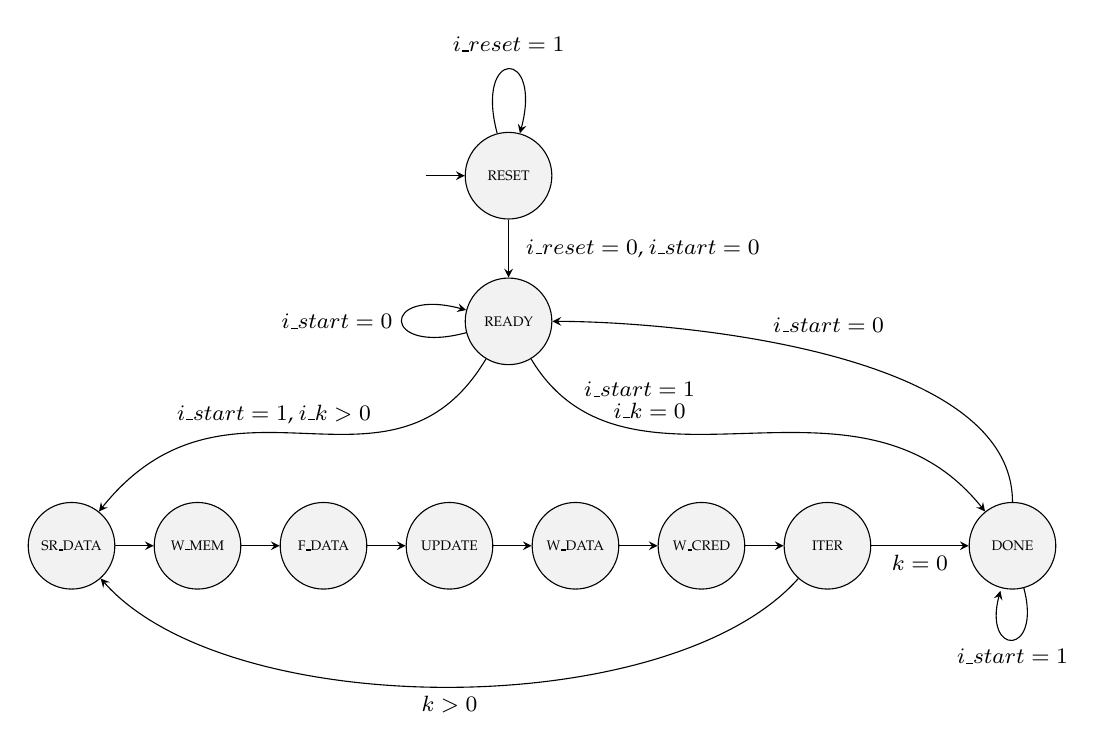
\begin{tikzpicture}[]
        \tikzset{
            ->,  % makes the edges directed
            >=stealth, % makes the arrow heads bold
            node distance=1.6cm, % specifies the minimum distance between two nodes. Change if n
            every state/.style={fill=gray!10, minimum size = 1.1cm}, % sets the properties for each ’state’ n
            initial text=$ $, % sets the text that appears on the start arrow
            }

        % nodes
        \node[state, initial] (reset_state) {\tiny RESET};
        \node[state, below of=reset_state, yshift=-0.25cm] (ready_state) {\tiny READY};
        \node[state, below of=ready_state, yshift=-1.25cm, xshift=-0.75cm] (update_state) {\tiny UPDATE};
        \node[state, left of=update_state] (fetch_data_state) {\tiny F\_DATA};
        \node[state, left of=fetch_data_state] (wait_mem_state) {\tiny W\_MEM};
        \node[state, left of=wait_mem_state] (set_read_data_state) {\tiny SR\_DATA};
        \node[state, right of=update_state] (write_data_state) {\tiny W\_DATA};
        \node[state, right of=write_data_state] (write_cred_state) {\tiny W\_CRED};
        \node[state, right of=write_cred_state] (iterate_state) {\tiny ITER};
        \node[state, right of=iterate_state, xshift=0.75cm] (done_state) {\tiny DONE};
    
        % reset state paths
        \path (reset_state) edge node [right, xshift=0.1cm] {\footnotesize \(i\_reset = 0\), \(i\_start = 0\)} (ready_state);
        \path (reset_state) edge [loop above, looseness=10] node [yshift=0.1cm] {\footnotesize \(i\_reset = 1\)} (reset_state);
        
        % ready state paths
        \draw (ready_state) .. controls ++(-1.5,-2.5) and ++(2,2.5) .. node [xshift=-0.4cm, yshift=0.25cm] {\footnotesize \(i\_start = 1\), \(i\_k > 0\)} (set_read_data_state);
        \path (ready_state) edge [loop left, looseness=10] node {\footnotesize \(i\_start = 0\)} (ready_state);
        \draw (ready_state) .. controls ++(1.5,-2.5) and ++(-2,2.5) .. node[right, pos=0.075, xshift=0.25cm] {\footnotesize \(i\_start = 1\)} node[right, pos=0.15, xshift=0.275cm] {\footnotesize \(i\_k = 0\)} (done_state);
%
        % done state paths
        \path (done_state) edge [loop below] node {\footnotesize \(i\_start = 1\)} (done_state);
        \draw (done_state) .. controls ++(0,2.5) and ++(2,0) .. node[pos=0.6, right, yshift=0.2cm] {\footnotesize \(i\_start = 0\)} (ready_state);
        
        % iterate state paths
        \path (iterate_state) edge node [midway, below] {\footnotesize \(k = 0\)} (done_state);
        \draw (iterate_state) .. controls ++(-2,-2.25) and ++(2,-2.25) .. node[midway, below] {\footnotesize \(k > 0\)} (set_read_data_state);
        
        % other states paths
        \path (set_read_data_state) edge (wait_mem_state);
        \path (wait_mem_state) edge (fetch_data_state);
        \path (fetch_data_state) edge (update_state);
        \path (update_state) edge (write_data_state);
        \path (write_data_state) edge (write_cred_state);
        \path (write_cred_state) edge (iterate_state);
    \end{tikzpicture}
    \caption{schema della FSM del modulo}
    \label{fig:my_label}
\end{figure}

\bigskip Per gli stati nella rappresentazione seguente della FSM, descritti con maggiore dettaglio nella sezione seguente, sono state utilizzate le seguenti abbreviazioni:

\begin{center}
    \begin{tabular}{l r}
        \texttt{SR\_DATA}: & \texttt{SET\_READ\_DATA} \\
        \texttt{W\_MEM}: & \texttt{WAIT\_MEM} \\
        \texttt{F\_DATA}: & \texttt{FETCH\_DATA} \\ 
        \texttt{W\_DATA}: & \texttt{WRITE\_DATA} \\
        \texttt{W\_CRED}: & \texttt{WRITE\_CREDIBILITY} \\
        \texttt{ITER}: & \texttt{ITERATE}
    \end{tabular}
\end{center}

\subsection{Stati}
Le operazioni compiute dal modulo in un ciclo di clock dipendono dallo stato in cui essa si trova. Gli stati utilizzati sono:
\begin{itemize}[label=\raisebox{0.25ex}{\tiny$\bullet$}]
    \item \texttt{\textbf{RESET}}: è lo stato iniziale e lo stato in cui il modulo si troverà dopo un segnale di reset in ingresso. Da specifica, la FSM rimarrà in questo stato fino a quando \texttt{i\_reset} e \texttt{i\_start} non verranno portati a 0. Se il segnale di start è già alto durante la transizione a 0 del segnale di reset, il modulo aspetterà un nuovo fronte di salita del primo;
    \item \texttt{\textbf{READY}}: è lo stato di idling. Il modulo rimane in attesa di un segnale di start;
    \item \texttt{\textbf{SET\_READ\_DATA}}: stato in cui il modulo comunica alla memoria la volontà di accedere in lettura ad essa, ad un determinato indirizzo \texttt{addr};
    \item \texttt{\textbf{WAIT\_MEM}}: la memoria fornita da specifica richiede un ciclo di clock in più per asserire in output i dati richiesti. Questo rende necessario che il modulo attenda un ulteriore ciclo di clock per far sì che i dati in ingresso siano quelli corretti;
    \item \texttt{\textbf{FETCH\_DATA}}: stato in cui il modulo recupera il dato dalla memoria;
    \item \texttt{\textbf{UPDATE}}: stato in cui il modulo esegue le operazioni a seconda dei dati letti.
    \item \texttt{\textbf{WRITE\_DATA}}: stato in cui il modulo scrive il dato nella memoria; 
    \item \texttt{\textbf{WRITE\_CREDIBILITY}}: stato in cui il modulo scrive il valore di credibilità nella memoria; 
    \item \texttt{\textbf{ITERATE}}: stato in cui i segnali interni vengono aggiornati e "preparati" per la prossima iterazione, sfruttando i segnali di \textit{next};
    \item \texttt{\textbf{DONE}}: stato che sancisce la fine dell'elaborazione. Il modulo esce da questo stato solamente all'alzarsi del segnale di \texttt{i\_start} in ingresso. Il modulo tornerà allo stato \texttt{READY}, abbassando il segnale di \texttt{o\_done}.
\end{itemize}

\vspace{0.75cm}
\subsection{Processi}
Il modulo è basato su due processi:
\begin{itemize}[label=\raisebox{0.25ex}{\tiny$\bullet$}]
    \item \texttt{\textbf{STATE\_REG}}: permette di aggiornare i segnali interni e lo stato della FSM. Nella lista di sensibilità sono presenti il segnale di reset e il segnale di clock.
    \\ Se il processo viene attivato dal segnale di reset, il modulo viene reimpostato azzerando tutti i segnali e gli output. Invece, se viene attivato da una variazione del segnale di clock, verifica se si tratta di un fronte di salita e, in tal caso, imposta tutti i segnali ai corrispondenti valori \textit{next}, compreso il segnale di stato. Questo processo modifica solo i segnali "correnti";
    \item \texttt{\textbf{LAMBDA\_DELTA}}: Il processo è composto da uno switch-case basato sullo stato corrente. Ogni case contiene le azioni da eseguire per lo specifico stato, in termini di aggiornamento sia dei segnali interni che degli output. Questo processo modifica solo i segnali \textit{next}.
\end{itemize}
É importante notare l'attenzione posta alle modifiche dei segnali interni per evitare errori riguardanti segnali "multiply driven", ossia segnali modificati concorrentemente da più processi.
\vspace{0.75cm}
\subsection{Segnali Interni}
\subsubsection{Segnali Correnti}
All'interno del modulo sono stati utilizzati diversi segnali per la gestione dell'elaborazione.
In particolare:
\begin{itemize}[label=\raisebox{0.25ex}{\tiny$\bullet$}]
    \item \texttt{\textbf{k}}: rappresenta il numero di parole che ancora devono essere elaborate. Posto a \texttt{i\_k} durante la fase di inizializzazione, viene decrementato ad ogni parola elaborata;
    \item \texttt{\textbf{addr}}: rappresenta l'indirizzo della memoria che il modulo sta elaborando. Inizialmente posto a \texttt{i\_add}, viene incrementato a ogni lettura/scrittura sulla memoria;
    \item \texttt{\textbf{data}}: rappresenta il dato letto all'iterazione corrente;
    \item \texttt{\textbf{last\_valid\_data}}: rappresenta l'ultimo valore specificato (i.e. diverso da zero) letto in memoria. Usato per aggiornare le celle in cui il dato non è specificato;
    \item \texttt{\textbf{credibility}}: rappresenta il valore di credibilità dell'ultimo dato valido letto. Viene decrementato ogni volta che l'ultimo dato valido viene scritto e reimpostato a 31 ogni volta che viene letto un nuovo dato.
\end{itemize}
\subsubsection{Segnali Successivi}
Per ogni segnale interno e di output sono anche inizializzati segnali di \textit{next}, in modo da tenere traccia del valore che i segnali stessi dovranno avere al ciclo di clock successivo.
\medskip \\
Ad ogni ciclo di clock, i segnali correnti vengono asseriti ai loro corrispondenti valori \textit{next}, opportunamente preparati per il nuovo stato.
\medskip \\
Questo design di implementazione permette di evitare l'utilizzo di latch non necessari.

\vspace{1.5cm}
\subsection{Schema Implementativo}
Di seguito lo schema implementativo, completo di RAM e segnali di input/output del modulo.

\vspace{0.25cm}
\begin{figure}[h]
    \centering
    \includegraphics[width=1\textwidth]{architecture.png}
\end{figure}

\newpage
\section{Risultati Sperimentali}
\subsection{Sintesi}
Si è scelto per l'implementazione di utilizzare la board target \texttt{\textbf{xc7a200tfbg484-1}}. Il modulo viene correttamente sintetizzato, rispettando la specifica e ottenendo risultati notevoli in termini di report, qui sotto elencati.
\subsubsection{Report di Utilizzo}
\begin{figure}[h]
    \centering
    \includegraphics[width=0.8\textwidth]{synth_report.png}
\end{figure}

Leggendo il report, possiamo notare che il modulo utilizza:
\begin{itemize}[label=\raisebox{0.25ex}{\tiny$\bullet$}]
    \item \texttt{\textbf{LUT}}: 76 (0.06\% del totale disponibile)
    \item \texttt{\textbf{FF}}: 87 (0.03\% del totale disponibile)
\end{itemize}

Una percentuale così bassa può essere spiegata dalla semplicità del problema da risolvere, che non richiede una logica complessa.
\smallskip \\ Durante la scrittura del codice è stata posta molta attenzione per evitare latch non necessari, portando così il loro numero a zero.

\subsubsection{Report di Timing}
Da specifica è richiesto che il modulo supporti un periodo di clock di \textit{almeno} 20 ns.

\begin{center}
    \begin{tabular}{l r}
        Slack: & MET \\
        Slack Time: & 16.206 ns \\
        Requirement: & 20.000 ns \\
        Data Path Delay: & 3.412 ns \\
        Logic: & 0.999 ns (29.279\%) \\
        Route: & 2.413 ns (70.721\%)
    \end{tabular}
\end{center}

Dal report leggiamo che il modulo rimane inattivo per più di 16 ns, ovvero più di quattro quinti del tempo disponibile.
Ne evinciamo che l'implementazione soddisfa ampiamente la specifica, con un percorso critico inferiore ai 4 ns. 

\bigskip
\subsection{Simulazioni}
\subsubsection{Overview}
Il codice è stato sviluppato seguendo una politica test-driven. I testbench elencati hanno permesso di scovare man mano criticità nel codice, risolte con versioni aggiornate dello stesso.
\smallskip \\ I testbench sono stati progettati appositamente per affrontare i punti critici, coprendo così tutti i possibili casi limite.
\smallskip \\ Sono di seguito elencate le macro sezioni, e per ognuna i singoli test effettuati.
\subsubsection{Casi limite di Segnali in Input e dei valori in Memoria}
    I casi di test sono stati progettati per verificare il corretto funzionamento del modulo sia in condizioni normali sia nei casi limite. Particolare cura è stata dedicata a:
    \begin{itemize}[label=\raisebox{0.25ex}{\tiny$\bullet$}]
        \setlength{\itemsep}{0pt}
        \item \texttt{i\_k} in ingresso pari a zero;
        \item cella all'indirizzo iniziale \texttt{i\_add} della memoria contenente zero;
        \item condizioni tali da portare il valore di credibilità a zero durante l'elaborazione;
        \item memoria contenente solo zeri.
    \end{itemize}
    I casi di test hanno permesso di confermare il codice già scritto in precedenza, non avendo portato a nessun errore in elaborazione.
\subsubsection{Asserimento di segnali di Reset e Start}
    Fondamentale è rispettare la specifica per quanto riguarda il funzionamento del modulo in caso di reset e di comandi di inizio di elaborazione. Si è voluto testare:
    \begin{itemize}[label=\raisebox{0.25ex}{\tiny$\bullet$}]
        \setlength{\itemsep}{0pt}
        \item segnale di start asserito prima del segnale di reset durante la fase iniziale;
        \item segnale di start mai abbassato dopo un segnale di reset;
        \item segnale di start asserito durante un segnale di reset;
        \item segnale di reset asserito durante la lettura in memoria.
    \end{itemize}
    I casi di test hanno rivelato un comportamento del modulo non conforme alla specifica: in presenza di un segnale di start durante un segnale di reset, il modulo iniziava l'elaborazione non appena il segnale di reset veniva azzerato.
    \medskip \\ Il codice è stato aggiornato affinché il modulo attenda un nuovo segnale di start ad ogni reset.
\subsubsection{Elaborazioni Multiple}
Il modulo deve essere in grado di gestire più elaborazioni successive, anche in assenza di segnali di reset. 

\subsubsection{Risultati}
La versione finale del modulo riesce a eseguire tutti i testbench senza difficoltà, sia in simulazione \textbf{behavioral} che in \textbf{post-synthesis functional}.
\medskip \\ Nonostante non fosse richiesto da specifica, si è deciso di simulare le elaborazioni anche in \textbf{post-synthesis timing}, tutte completate con successo. 

\newpage
\section{Conclusioni}
\subsection{Contesto}
La specifica sembra descrivere un problema quale potrebbe essere l'acquisizione di grandezze esterne attraverso, per esempio, strumenti di sensoristica. Ad ogni quanto di tempo, se il sensore ha letto un valore diverso da quello precedente, lo scrive in memoria, altrimenti non specifica il valore.
\medskip \\ Per questo motivo è richiesto il valore di credibilità, una metrica che permette di conoscere quanto tempo prima un determinato valore è stato acquisito, ergo quanto è attendibile.
\subsection{Implementazione}
Si ritiene innanzitutto che l'implementazione del modulo rispetti le specifiche.
\medskip \\ L'utilizzo di una FSM per gestire il flusso dell'elaborazione ha permesso di semplificare in maniera non ininfluente sia la complessità della computazione che la leggibilità del codice. 
\medskip \\ E' comunque necessario notare come potrebbero essere apportate alcune modifiche volte a migliorare ancor più l'implementazione.
\medskip \\ In primo luogo, la FSM non è stata ottimizzata in termini di numero di stati in quanto non ritenuto necessario per il livello di complessità del problema; si è invece preferito mantenere più chia\-rezza e una maggiore divisione di responsabilità.
\medskip \\ In secondo luogo, il numero di Flip Flop utilizzati per sintetizzare il componente potrebbe essere ridotto leggermente riducendo il numero di segnali interni; anche in questo caso non lo si è considerato necessario vista la natura del problema.
\end{document}